\documentclass[tikz]{standalone}
\usetikzlibrary{arrows}
\usetikzlibrary{arrows.meta}

\tikzset{
%Define standard arrow tip
>=latex',
%Define style for different line styles
%help lines/.style={dashed, thick},
%axis/.style={<->},
%important line/.style={thick},
%connection/.style={thick, dotted},
}

\begin{document}
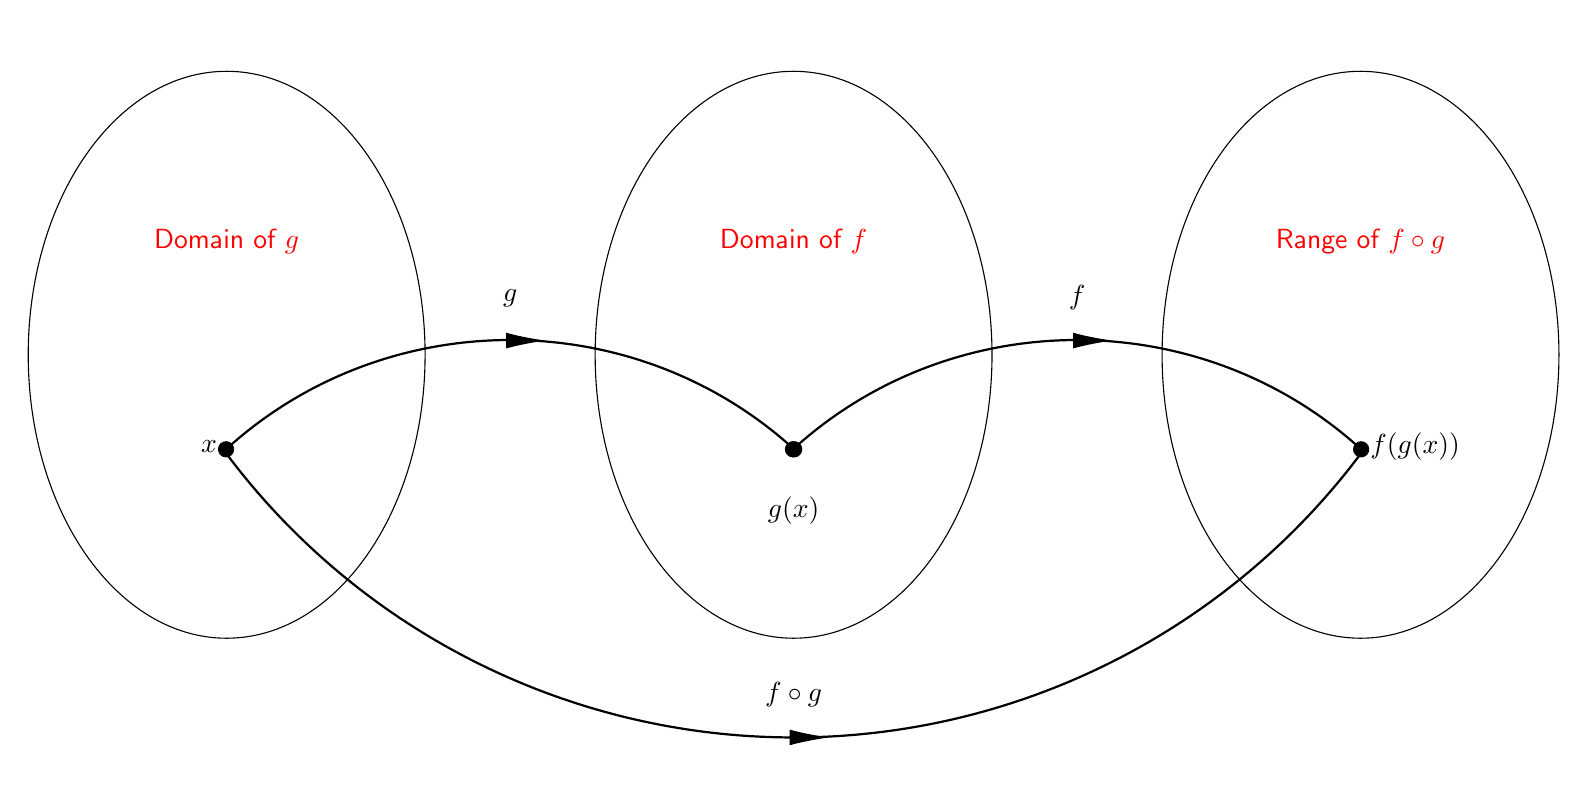
\begin{tikzpicture}[scale=1.8]

% create a white background, with a black frame
%\draw [fill=white] (-6,-4) rectangle (6,4);  % black border

% g
\draw[fill=white] (2,4) ellipse [x radius = 1.4cm, y radius = 2cm];
%\node at (-6,2) {\Large $A$};
\node[red] at (2,4.8) {\sffamily Domain of $g$};

%% domain f(g)
%\draw[fill=white] (2,3.5) ellipse [x radius = 1.2cm, y radius = 1.5cm];
%\node[red] at (2,4) {\sffamily Domain of $f\circ g$};
\node[left] at (2,3.35) {$x$};

% f
\draw[fill=white] (6,4) ellipse [x radius = 1.4cm, y radius = 2cm];
%\node at (0,2) {\Large $B$};
\node[red] at (6,4.8) {\sffamily Domain of $f$};
\node at (6,2.9) {$g(x)$};

% range f(g)
\draw[fill=white] (10,4) ellipse [x radius = 1.4cm, y radius = 2cm];
%\node at (6,2) {\Large $B$};
\node[red] at (10,4.8) {\sffamily Range of $f\circ g$};
\node[right] at (10,3.35) {$f(g(x))$};


\draw[*-*,thick] (4,1.1) +(47:3) arc (47:133:3);
\node at (4,4.4) {$g$};
\draw[-{Latex[length=5mm,width=2mm]}] (4.15,4.1) -- (4.25,4.1);
%\draw[-{Latex[length=5mm,width=2mm]}] (-3,-5) +(90:5) arc (90:86:5);

\draw[*-*,thick] (8,1.1) +(47:3) arc (47:133:3);
\node at (8,4.4) {$f$};
\draw[-{Latex[length=5mm,width=2mm]}] (8.15,4.1) -- (8.25,4.1);
%\draw[-{Latex[length=5mm,width=2mm]}] (3,-5) +(90:5) arc (90:86:5);

\draw[thick] (6,6.3) +(217:5) arc (217:323:5);
\draw[-{Latex[length=5mm,width=2mm]}] (6.15,1.3) -- (6.25,1.3);
\node at (6,1.6) {$f\circ g$};

\end{tikzpicture}
\end{document}
